\section{Allgemeines Programmiermodell}
Dieser Abschnitt soll dazu dienen einen allgemeinen "Uberlick "uber die Assemblerprogrammierung zu erhalten, da sich die Programmiermodelle unter den Mikroprozessoren variieren.
\subsection{Begriffserkl"arung}
\begin{minipage}{10cm}
	Der Mikroprozessor stellt den Anwender zur Programmierung den \textbf{Maschincode} zur Verf"ugung. Der Maschinencode besteht aus \textbf{Bitfolgen}, welche das Steuerwerk des Prozessors als Befehle interpretiert, auswertet und danach Aktionen ausf"uhrt. Die einzelnen Befehle sind bin"ar codiert und werden aus dem \textbf{Programmspeicher} heraus der CPU zur Ausf"uhrung bereitgestellt.\\
	
	Die \textbf{Assemblersprache} ist eine maschinenorientierte Sprache. Durch Abk"urzungen (\textbf{Mnemonics}) wird das Programmieren vom bin"are Maschinencode erleichtert.\\
	
	Das \textbf{Assemblier-Program} "ubersetzt Assembler Sprache in bin"aren Maschinencode.\\
	
	Bei der hardwarenahen Programmierung verwendet der Programmierer das \textbf{Registermodell} und \textbf{Befehlssatz} des verwendeten Prozessors.
\end{minipage}
%
\begin{minipage}{0.5cm}
	\ \
\end{minipage}
%
\begin{minipage}{8cm}
	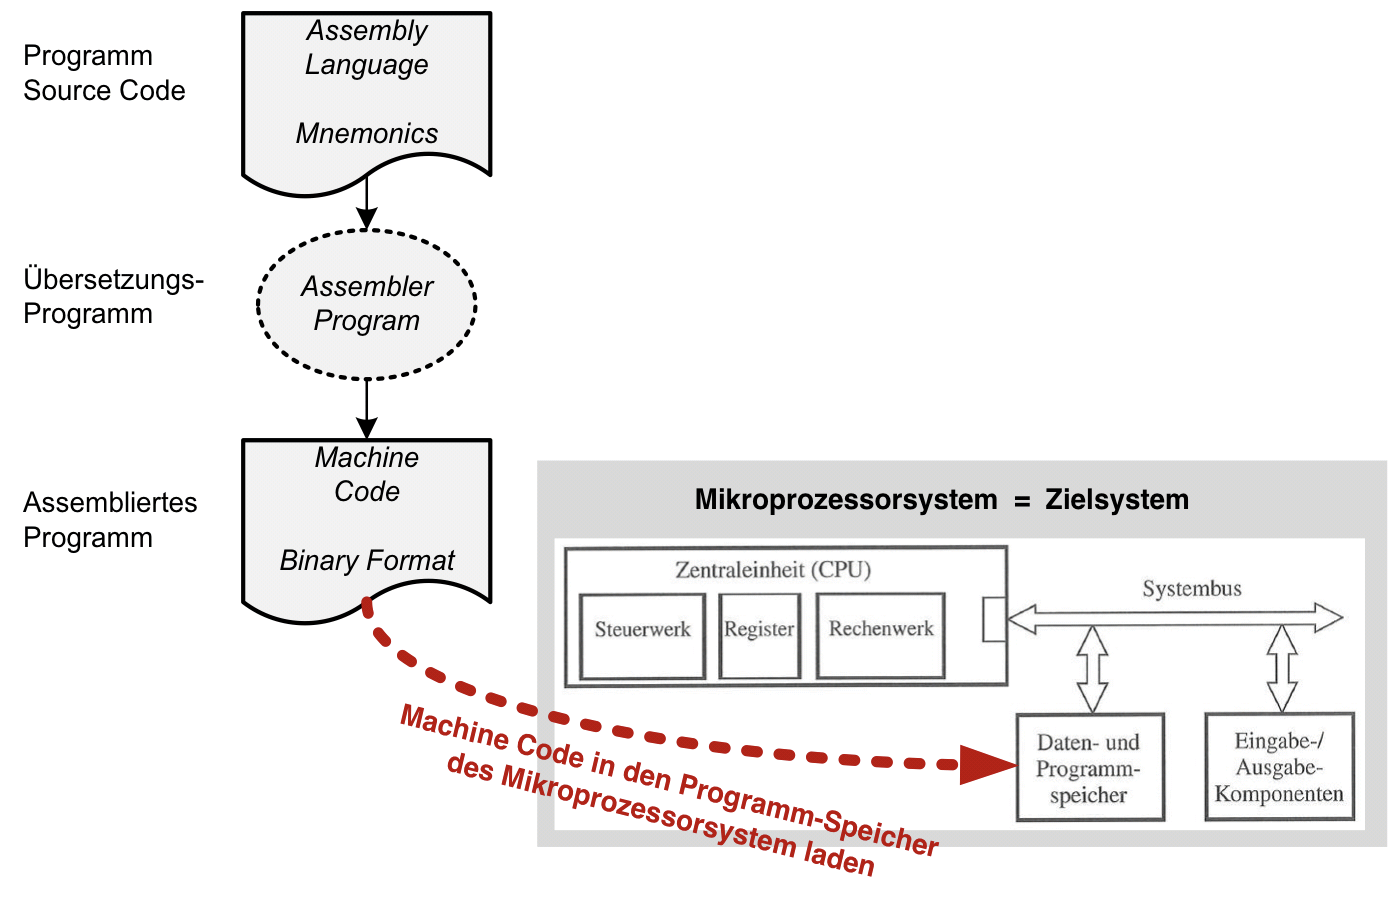
\includegraphics[width = 8cm]{pics/Programmiermodell}
\end{minipage}
	
\subsection{Registersatz}
Als \textbf{Registersatz} bezeichnet man die mittels Maschinenbefehle direkt ansprechbaren Register eines Mikroprozessors.

\subsection{Adressierungsarten}
Die Adressierungsart ist der Algorithmus, wie eine Adresse eines Operanden berechnet wird. Durch den geschickten Einsatz von Adressierungsarten k"onnen Programmieraufgaben effizient und elegant gel"ost werden.

\subsubsection{Unmittelbare Adressierung (Immediate Addressing)}
Bei dieser Adressierungsart ist der betroffene Operand eine Konstante, die im Anschluss am dem OpCode im Speicher steht.
\begin{minipage}{2cm}
	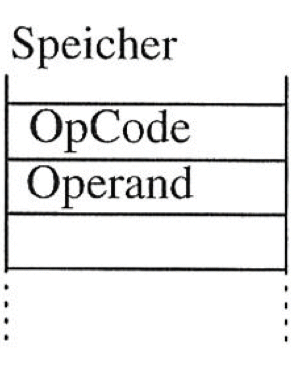
\includegraphics[width=2cm]{pics/Unmittelbare-Adressierung}
\end{minipage}
%
\begin{minipage}{0.5cm}
	\ \
\end{minipage}
%
\begin{minipage}{9cm}
	\textbf{Beispiel:}\\
	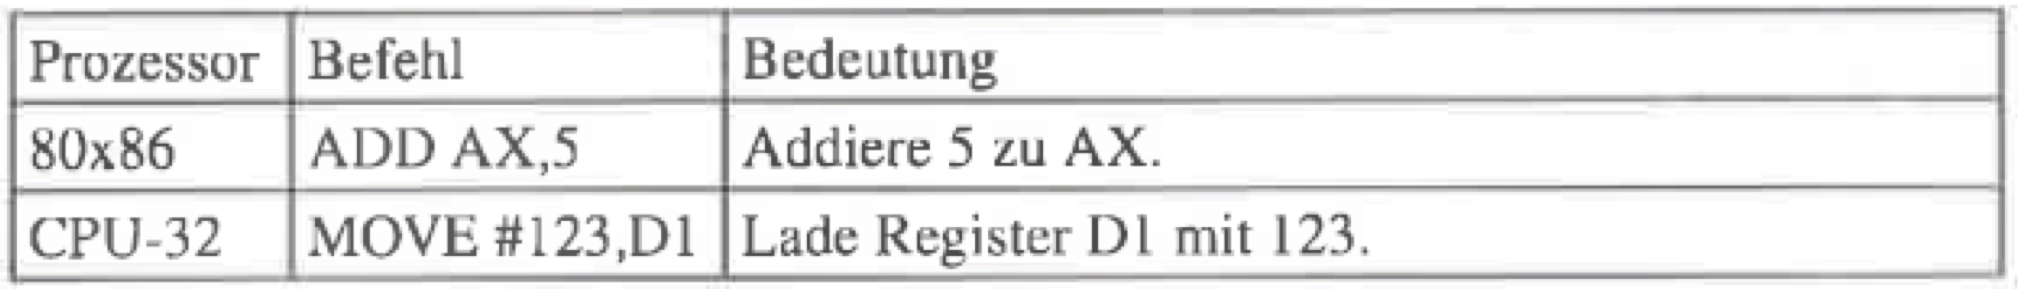
\includegraphics[width=9cm]{pics/UnmittelbareAdressierung-Bsp}
\end{minipage}

\subsubsection{Absolute Adressierung (Direct Addressing, Absolute Addressing)}
Ein absolut adressierter Operand ist ein Wert an einer bestimmten Speicheradresse, die im Befehl mit angegeben wird.
\begin{minipage}{4cm}
	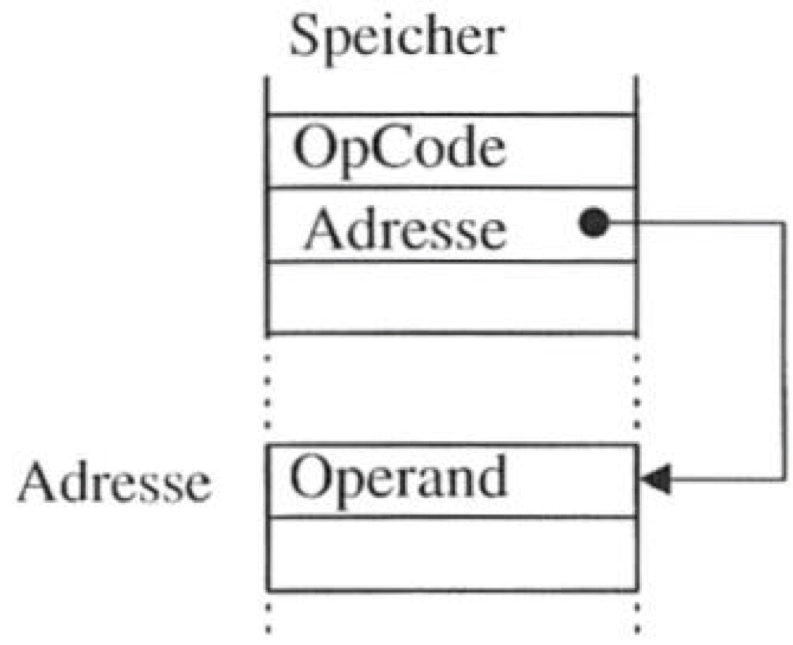
\includegraphics[width=4cm]{pics/Absolute-Adressierung}
\end{minipage}
%
\begin{minipage}{0.5cm}
	\ \
\end{minipage}
%
\begin{minipage}{9cm}
	\textbf{Beispiel:}\\
	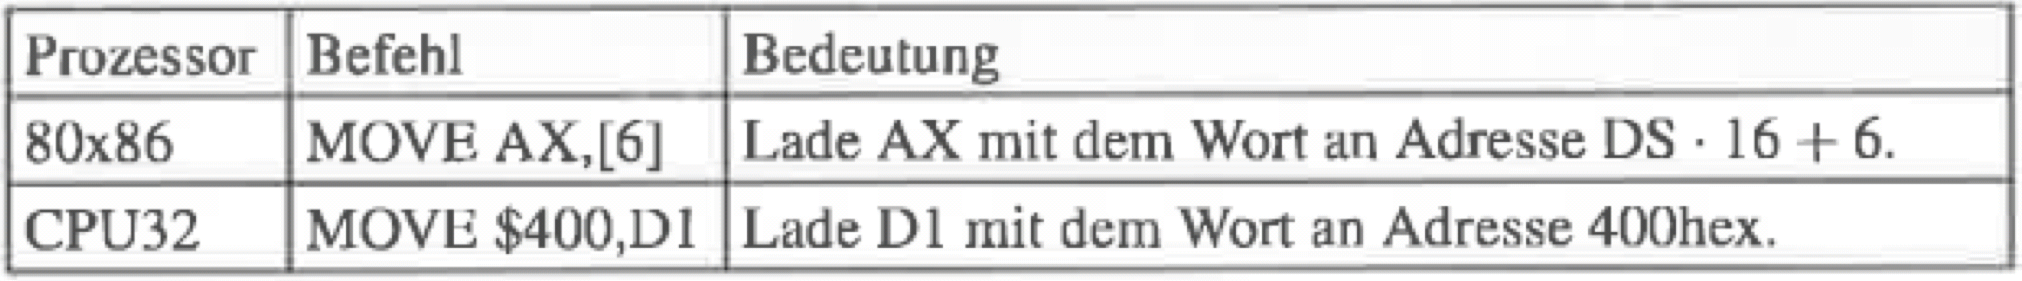
\includegraphics[width=9cm]{pics/Absolute-Adressierung-Bsp}
\end{minipage}

\subsubsection{Explizite Register Adressierung (Register Direct Addressing)}
Bei der expliziten Register Adressierung ist der Operand Inhalt eines Prozessorregisters. Es k"onnen universelle Register, Datenregister, Adressregister und auch spezielle Register wie Stackpointer und Statusregister angesprochen werden.
\begin{minipage}{5cm}
	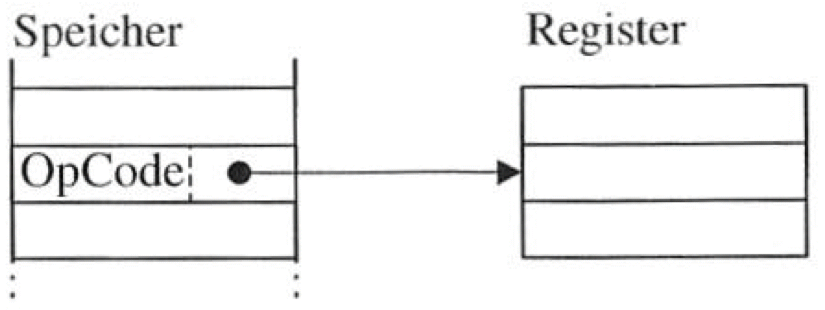
\includegraphics[width=5cm]{pics/Explizite-Adressierung}
\end{minipage}
%
\begin{minipage}{0.5cm}
	\ \
\end{minipage}
%
\begin{minipage}{9cm}
	\textbf{Beispiel:}\\
	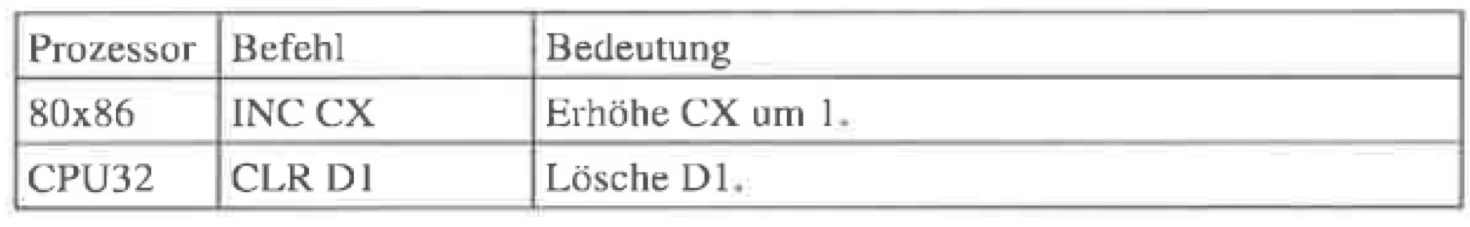
\includegraphics[width=9cm]{pics/Explizite-Adressierung-Bsp}
\end{minipage}

\subsubsection{Indizierte Adressierung (Indexed Addressing)}
Wird anstatt einer konstanten eine variable Adressdistanz ben"otigt, die erst zur Laufzeit eines Programmes feststeht, so wird die \textbf{indizierte Adressierung} verwendet.\\
Die effektive Adresse wird hier aus der Basisadresse (A1) in einem Adressregister und einem Adressversatz aus einem weiteren Register berechnet. Bei manchen Prozessoren ist daf"ur ein spezielle Indexregister vorhanden.

\begin{minipage}{7cm}
	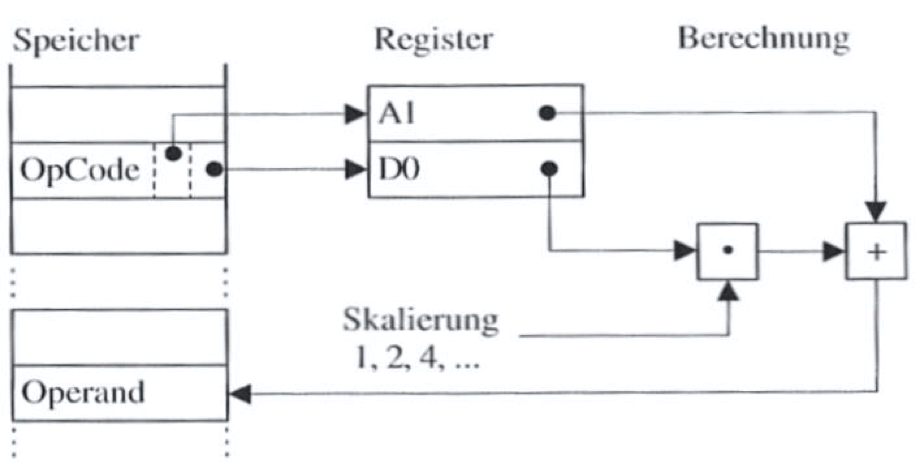
\includegraphics[width=7cm]{pics/Indizierte-Adressierung}
\end{minipage}
%
\begin{minipage}{0.5cm}
	\ \
\end{minipage}
%
\begin{minipage}{9cm}
	\textbf{Beispiel:}\\
	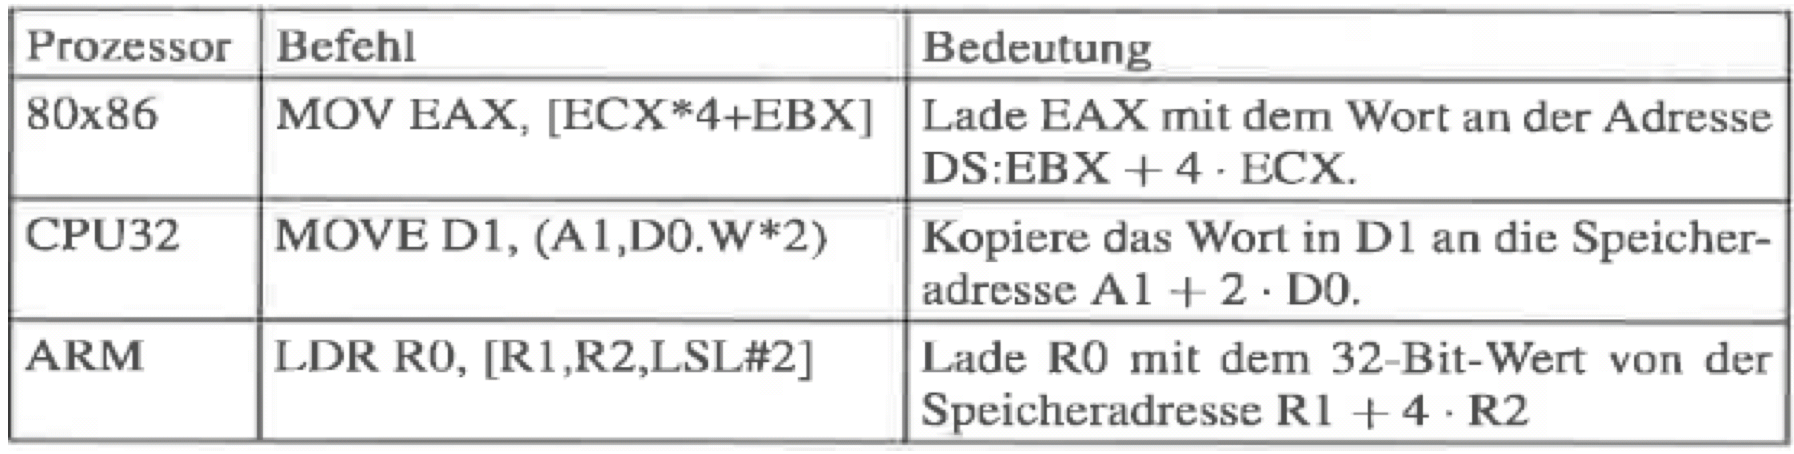
\includegraphics[width=9cm]{pics/Indizierte-Adressierung-Bsp}
\end{minipage}

\subsubsection{Implizite Register Adressierung (Implied Register Addressing)}
\begin{minipage}{9cm}
	Einige Befehle benutzen \textbf{implizite Operanden}, d.h. eine ausdr"uckliche Angabe der Operanden ist gar nicht erforderlich. Der Kontext des Befehls definiert die erforderlichen Operanden vollst"andig.  So verwenden beispielsweise einige arithmetische Befehle implizit den Akkumulator oder ein anderes Register.
\end{minipage}
%
\begin{minipage}{0.5cm}
	\ \
\end{minipage}
%
\begin{minipage}{9cm}
	\textbf{Beispiel:}\\
	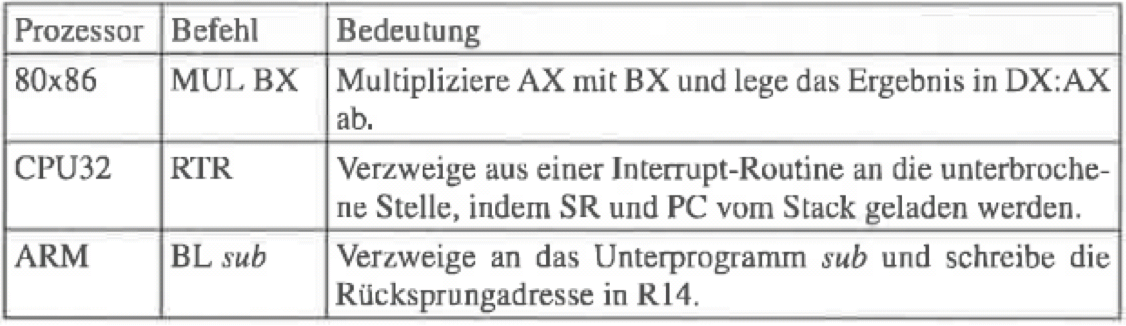
\includegraphics[width=9cm]{pics/Implizite-Register-Adressierung-Bsp}
\end{minipage}

\subsection{Befehlssatz/Befehlsgruppen}
Der \textbf{Befehlssatz (Instruction Set)} umfasst alle Maschinenbefehle, welche der Mikroprozessor ausf"uhren kann. Der Befehlssatz ist dem Aufbau und der Prozessorarchitektur angepasst.\\
Der Befehlssatz ist in einer \textbf{Befehlsliste} spezifiziert.

\subsection{Debug-Unterst"utzung}
Die meisten Prozessoren bieten als Debug-Unterst"utzung den \textbf{Trap-Mechanismus} an. Dabei wird bei der Ausf"uhrun eines Befehls eine Unterbrechungsroutine aufgerufen, die dann die Auswirkungen des Befehls interpretieren und anzeigen kann.\\
Verschiedene Prozessoren bieten dar"uber hinaus weitergehende Features an.

\subsection{Einf"uhrung in die Programmierung}
Der \textbf{Befehlssatz} eines Prozessors ist die Menge der Befehlscodes, die der jeweilige Prozessor direkt, d.h. ohne weitere Konvertierung oder Interpretierung ausf"uhren kann.

\textbf{Mnemonics:} Aus einpr"agsamen Abk"urzungen zusammengesetzte Befehlscodes

\textbf{Assemblierung:} "Ubersetzung von Assemblersprache in Maschinensprache 

\textbf{Disassemblierung:} "Ubersetzung von Maschinensprache in Assemblersprache 

\subsubsection{Code-Beispiel}
\begin{minipage}[t]{6cm}
	\textbf{Grundlegender Programmablauf:}\\
	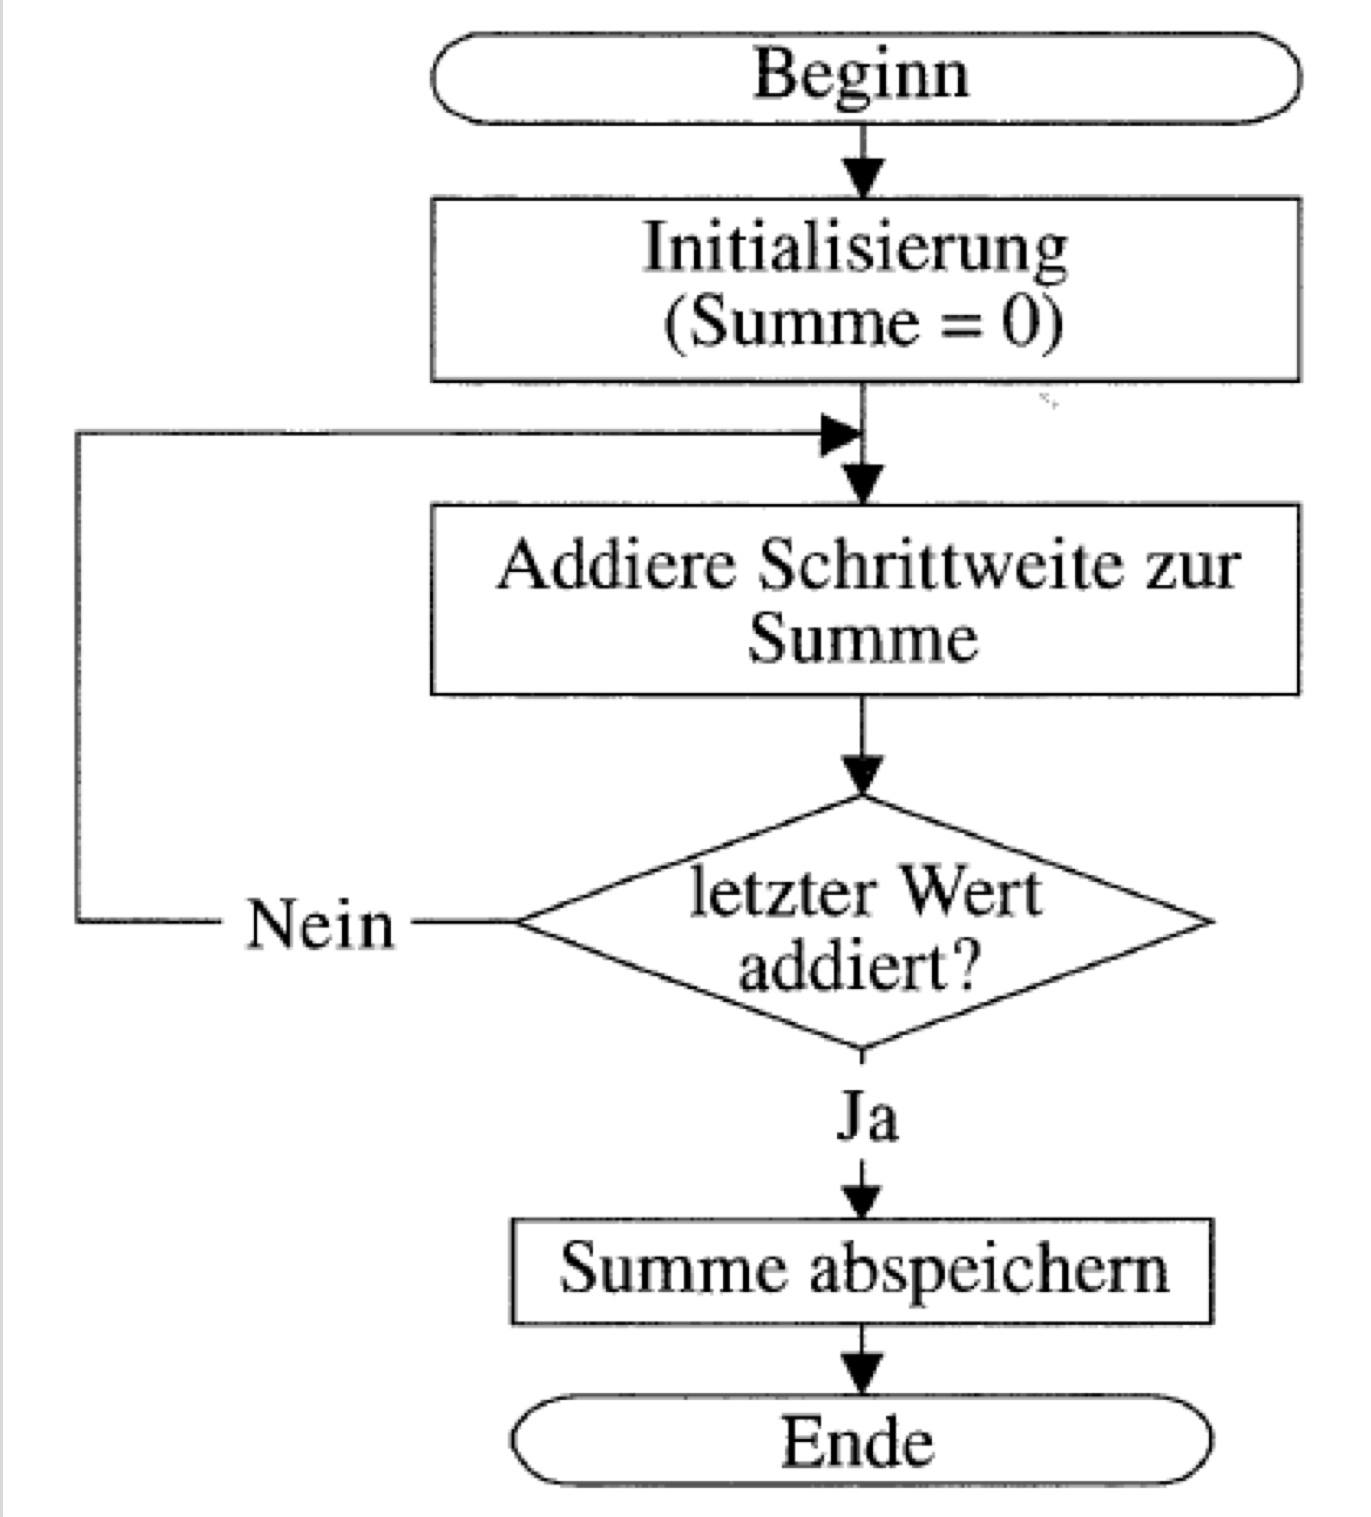
\includegraphics[width=6cm]{pics/Bsp-Programmablauf}
\end{minipage}
%
\begin{minipage}{0.25cm}
	\ \
\end{minipage}
%
\begin{minipage}[t]{6cm}
	\textbf{Assemblerprogramm 68000:}\\
	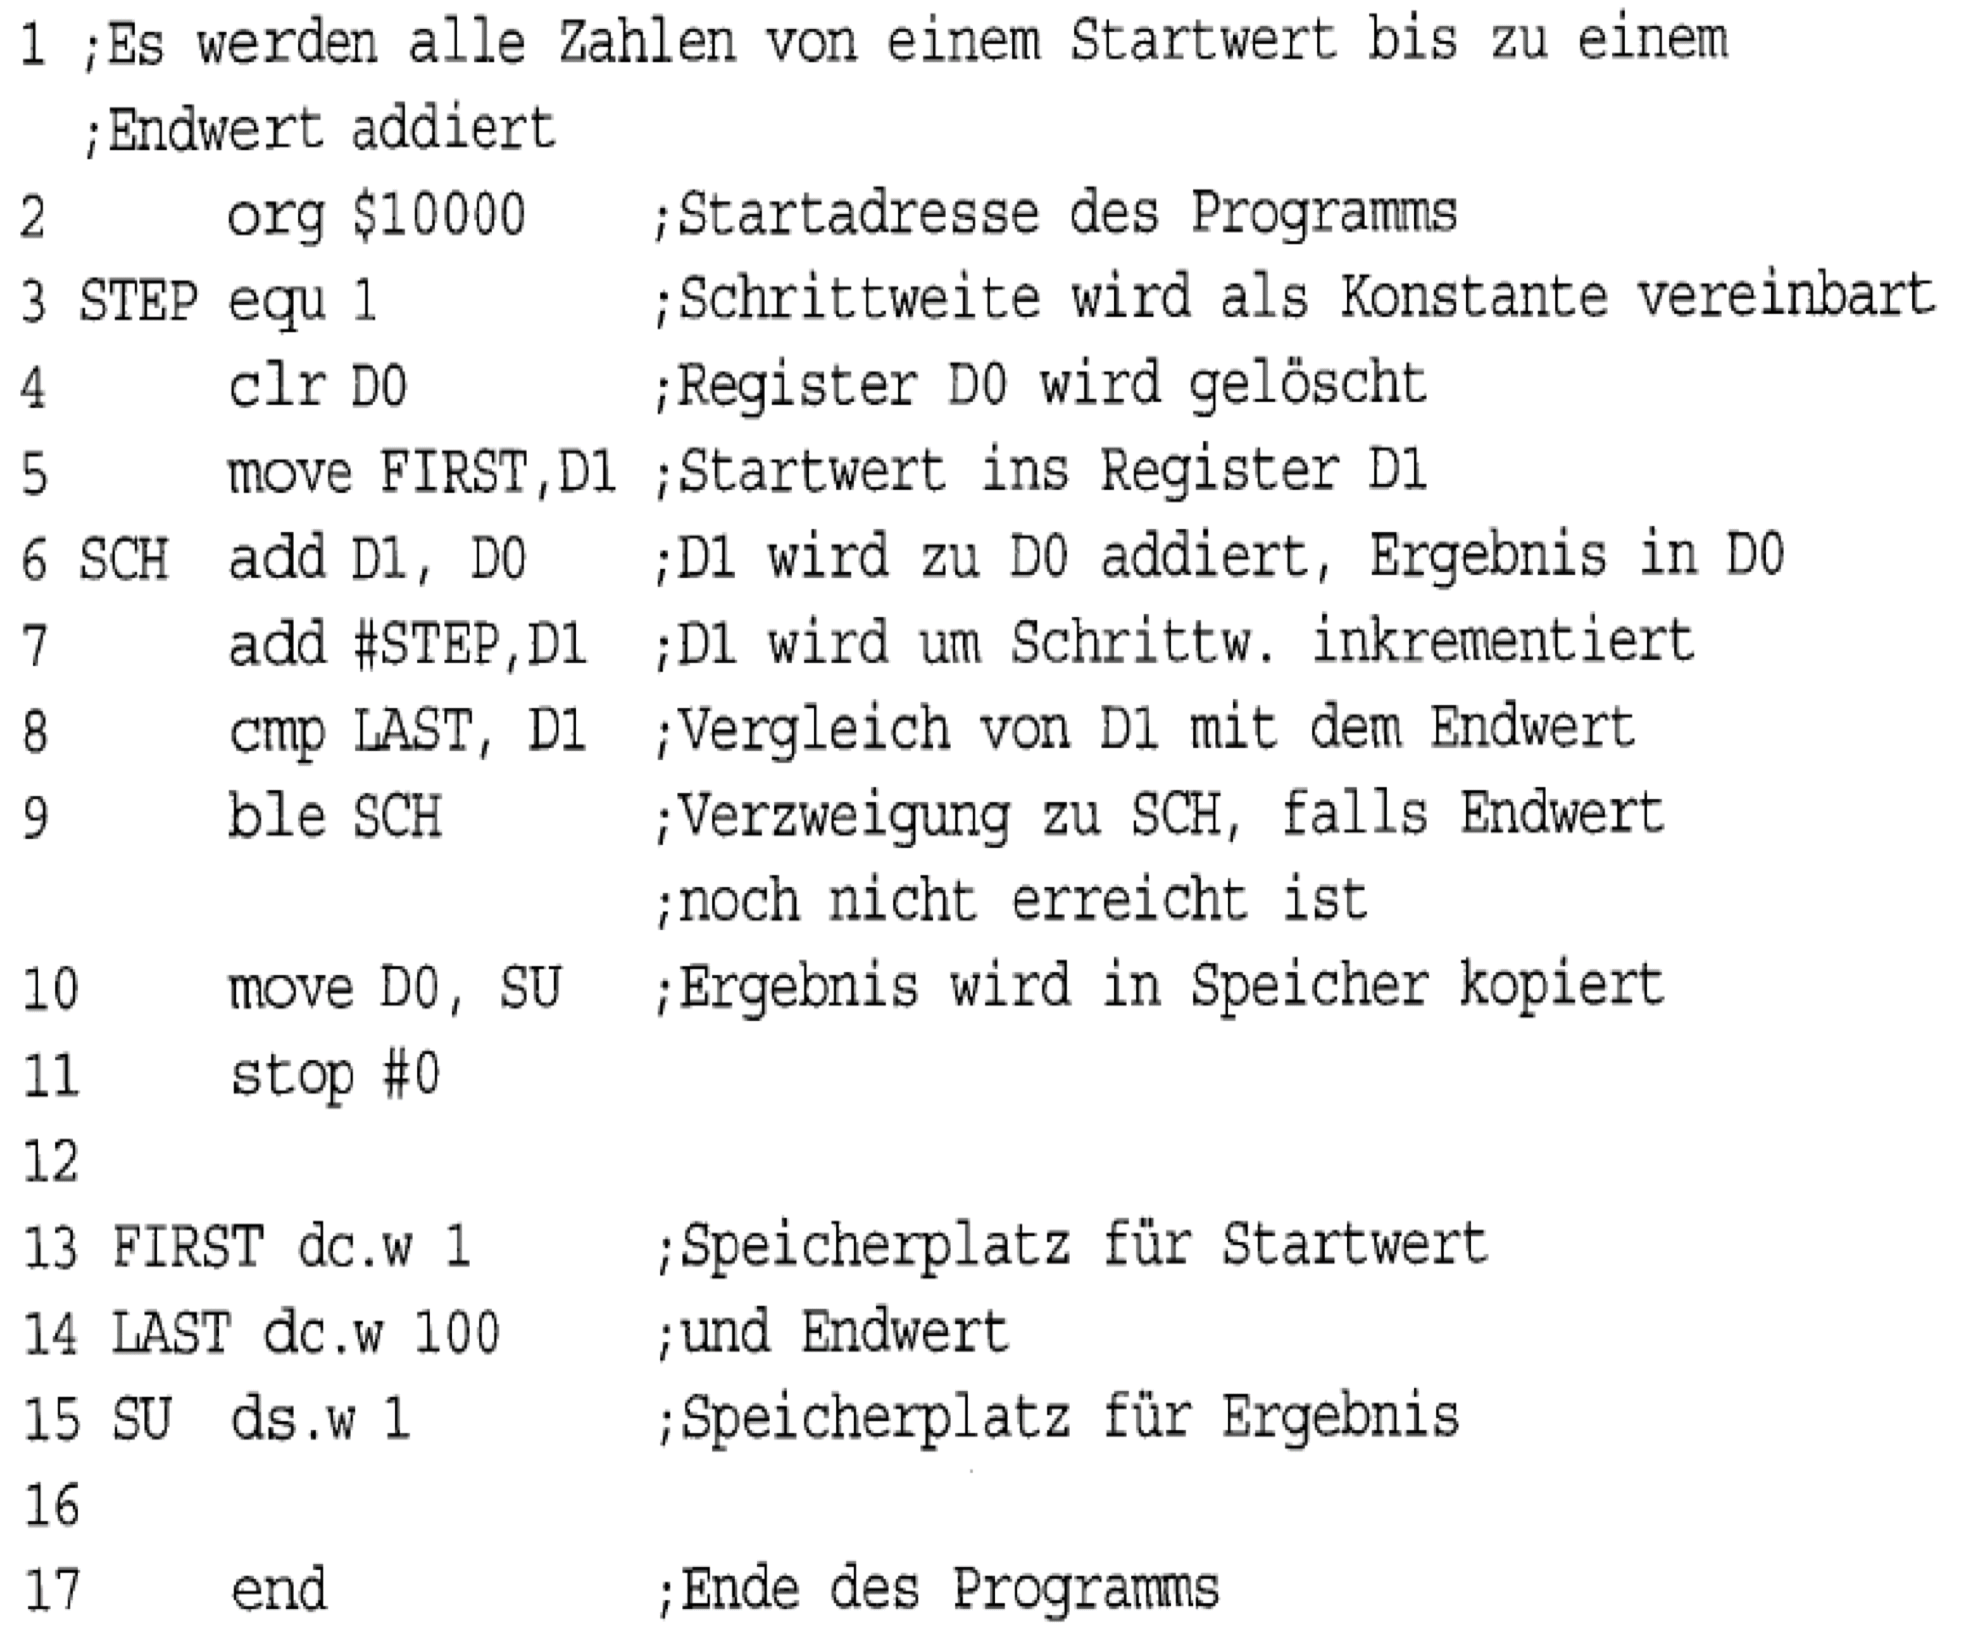
\includegraphics[width=6cm]{pics/Bsp-Assembler}
	
\end{minipage}
%
\begin{minipage}{0.25cm}
	\ \
\end{minipage}
%
\begin{minipage}[t]{6cm}
	\textbf{Maschinencode im Speicher:}\\
	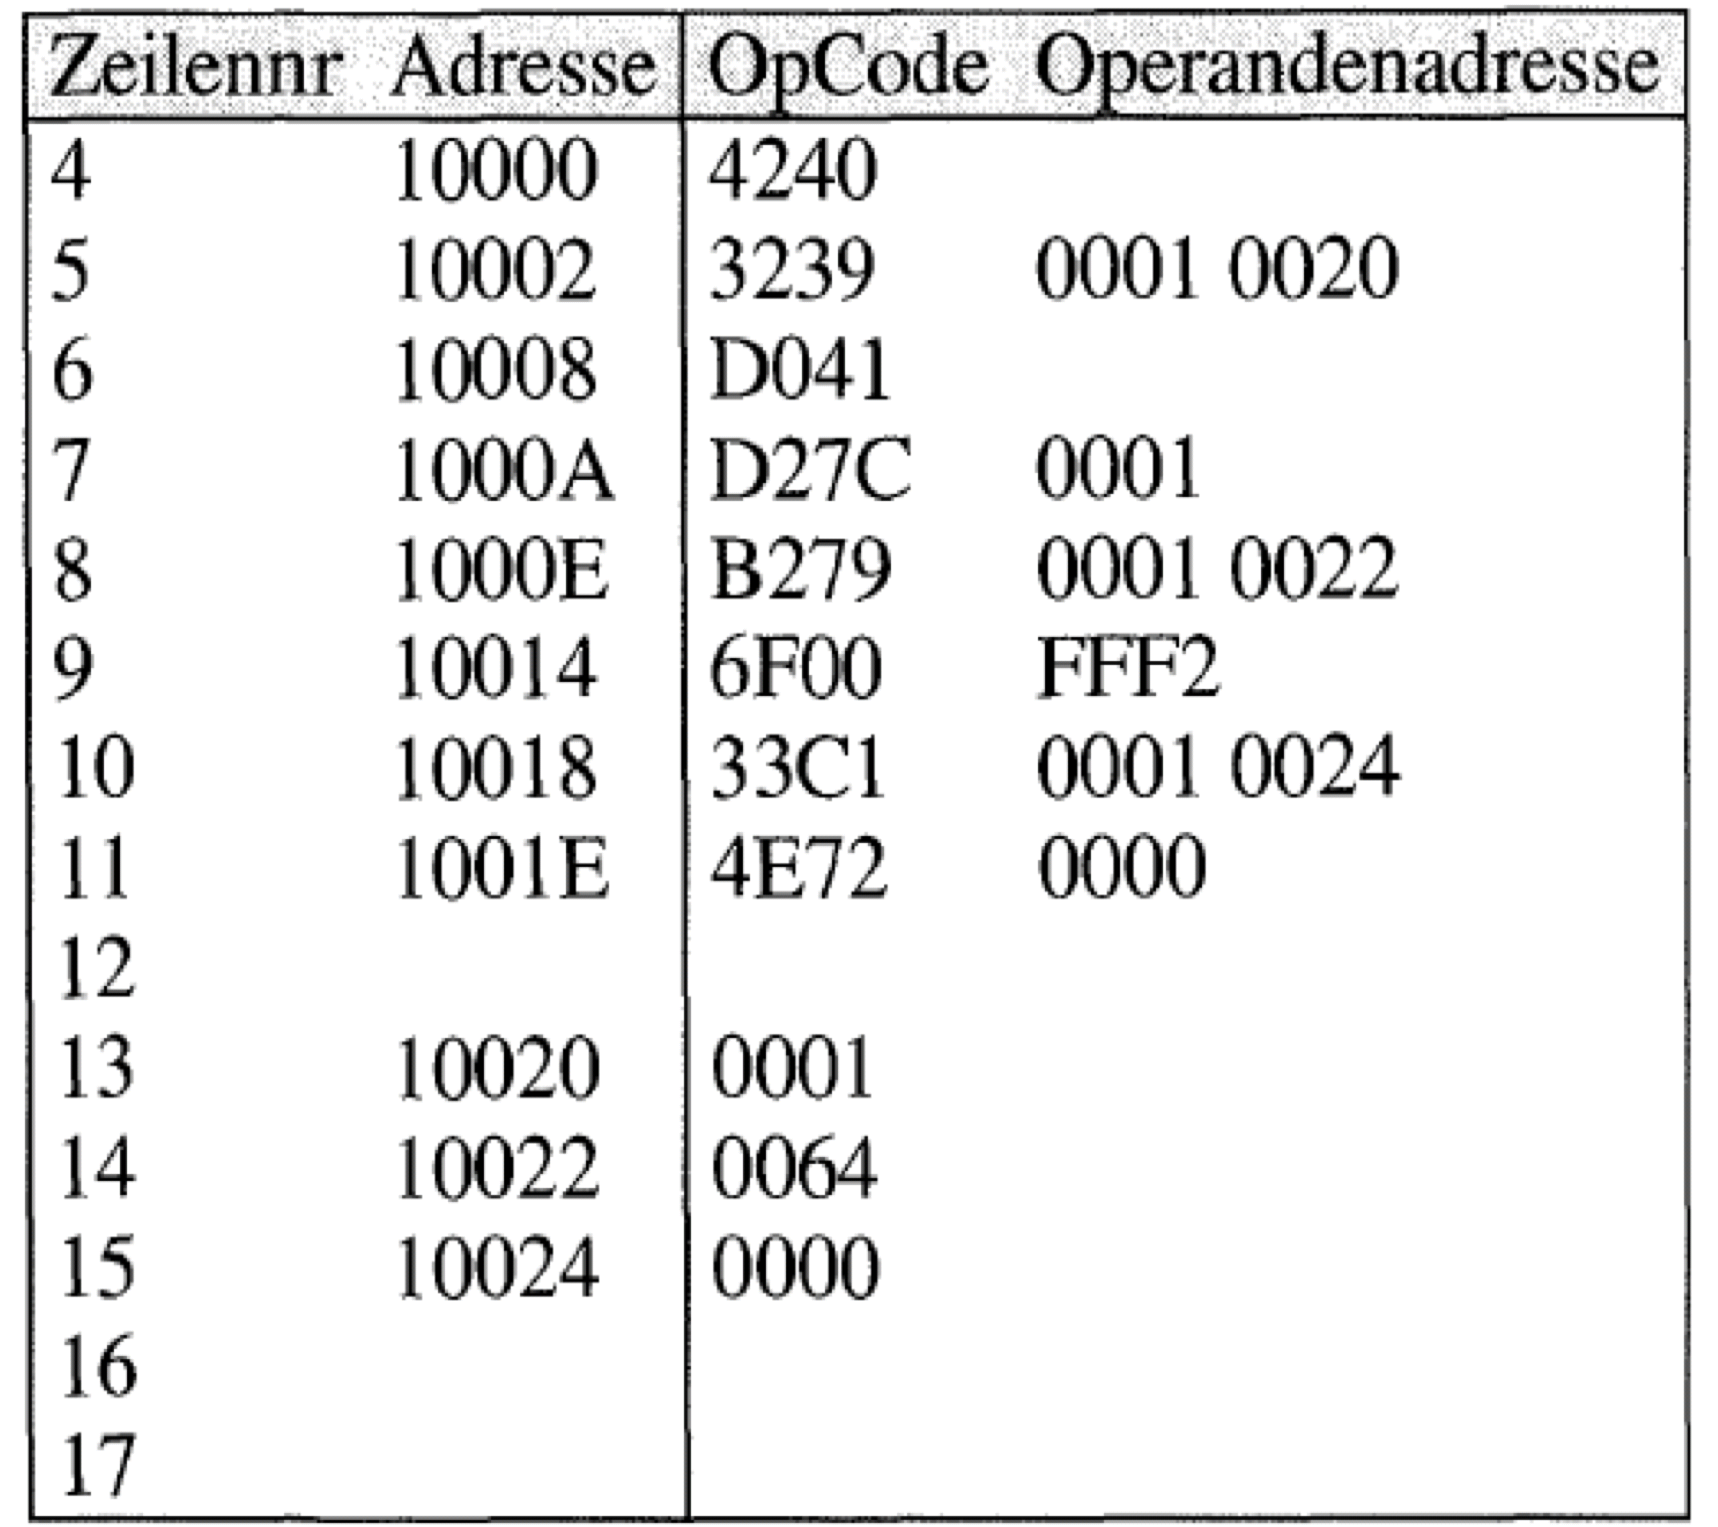
\includegraphics[width=6cm]{pics/Bsp-Maschinencode}
\end{minipage}